\documentclass{beamer}
\usepackage[utf8]{inputenc}
\usepackage[T1]{fontenc}
\usepackage{mathabx}
\usepackage{mathpazo}
\usepackage{eulervm}
\usepackage{natbib}
\usepackage{enumerate}
\usepackage{mathrsfs}

\usetheme{Madrid}
\usefonttheme{structurebold}
\usecolortheme{dove}
\title{VE401 RC Week4}
\author{Wang Yangyang}
\date{2022 Spring}
\institute{UM-SJTU JI}
\setbeamersize{text margin left = 20pt, text margin right = 20pt}

\AtEndDocument{\begin{frame}{End}

                  Credit to Zhanpeng Zhou (TA of SP21)
                  
                  Credit to Fan Zhang (TA of SU21)
                  
                  Credit to Jiawen Fan (TA of SP21)
                  
                  Credit to Zhenghao Gu (TA of SP20)
                  
                  \url{https://www.johndcook.com/blog/distribution_chart/}
               \end{frame}
                }
                
\definecolor{antiquefuchsia}{rgb}{0.57, 0.36, 0.51}
\newcommand{\bb}[1]{\textcolor{antiquefuchsia}{\textbf{\textit{#1}}}}

\begin{document}
\maketitle

\begin{frame}
\frametitle{Outline}
\tableofcontents
\end{frame}

%\AtBeginSection[ ]
%{
%\begin{frame}{Outline for \secname}
%	\tableofcontents[currentsection, hideothersubsections, %sectionstyle=show/show]
%\end{frame}
%}

\AtBeginSubsection[]{
  \frame<beamer>{ 
    \frametitle{Outline}   
    \tableofcontents[currentsection,currentsubsection] 
  }
}

\section{Distributions of Continuous Random Variables}
\subsection{Exponential, Gamma, Chi-Squared Distribution (Done)}
\begin{frame}{Connections}
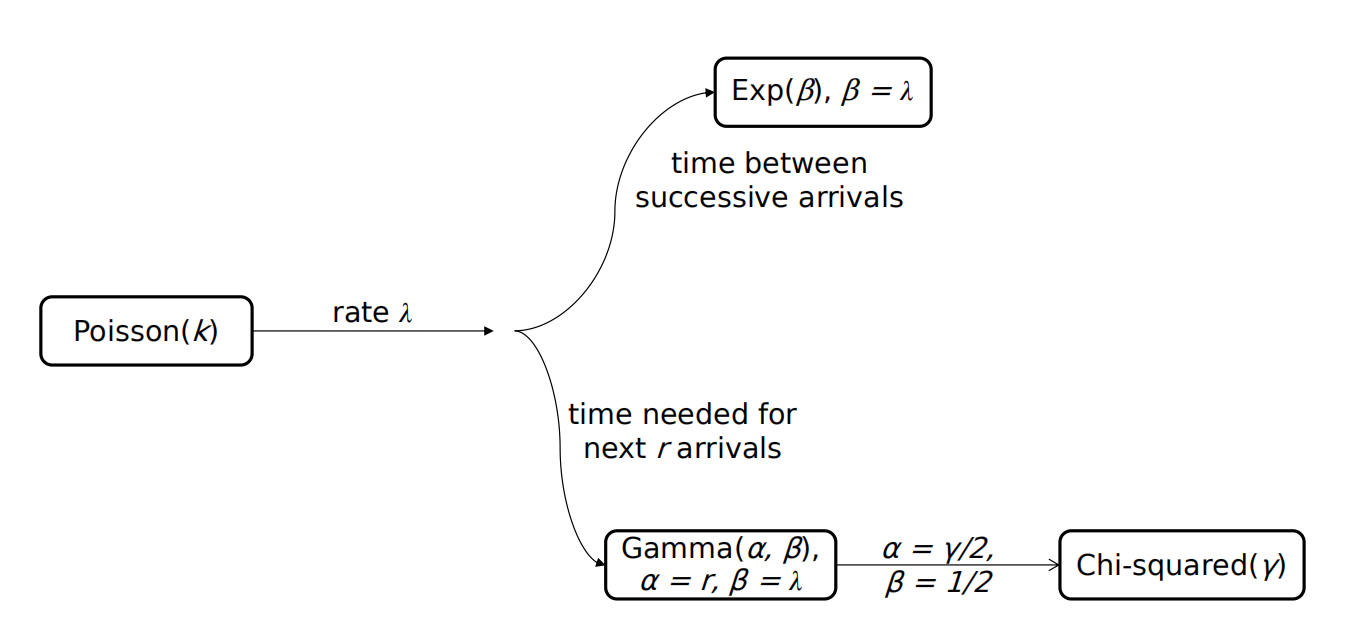
\includegraphics[scale=0.35]{connection.png}
\end{frame}

\subsection{Normal Distribution}
\begin{frame}{Normal Distribution}
\begin{block}{Definition}
A continuous random variable $\left(X, f_{\mu, \sigma^{2}}\right)$ has the \bb{normal distribution} with mean $\mu \in \mathbb{R}$ and variance $\sigma^{2}, \sigma>0$ if the probability density function is given by
$$
f_{\mu, \sigma^{2}}=\frac{1}{\sqrt{2 \pi \sigma^{2}}} \exp \left[-\frac{1}{2}\left(\frac{x-\mu}{\sigma}\right)^{2}\right], \quad x \in \mathbb{R}
$$
\end{block}
\end{frame}

\begin{frame}{Normal Distribution}
\begin{block}{Properties}
\begin{itemize}
\item Mean.
$$
\mathrm{E}[X]=\mu
$$
\item Variance.
$$
\operatorname{Var}[X]=\sigma^{2}
$$
\item M.G.F.
$$
m_{X}: \mathbb{R} \rightarrow \mathbb{R}, \quad m_{X}(t)=\exp \left(\mu t+\frac{1}{2} \sigma^{2} t^{2}\right)
$$
\end{itemize}
\end{block}
Let's verify the moment-generating function and see what's the takeaway from it.
\end{frame}

\begin{frame}{Normal Distribution}
\begin{block}{Proof}
$$
\begin{aligned}
m_{X}(t) &=E\left[e^{t X}\right]=\int_{-\infty}^{\infty} \frac{e^{t x}}{\sqrt{2 \pi} \sigma} e^{-((x-\mu) / \sigma)^{2} / 2} \mathrm{~d} x \\
&=\frac{1}{\sqrt{2 \pi} \sigma} \int_{-\infty}^{\infty} e^{\mu t+\sigma^{2} t^{2} / 2} \cdot e^{-\frac{\left(x-\left(\mu+\sigma^{2} t\right)\right)^{2}}{2 \sigma^{2}}} \mathrm{~d} x \\
&=e^{\mu t+\sigma^{2} t^{2} / 2} \underbrace{\frac{1}{\sqrt{2 \pi} \sigma} \int_{-\infty}^{\infty} e^{-\frac{\left(x-\left(\mu+\sigma^{2} t\right)\right)^{2}}{2 \sigma^{2}}}}_{=1} \mathrm{~d} x \\
&=e^{\mu t+\sigma^{2} t^{2} / 2}
\end{aligned}
$$
\end{block}
\end{frame}


\begin{frame}{Normal Distribution}
\begin{block}{Proof}
To verify that
$$
I:=\int_{-\infty}^{\infty} e^{-\frac{(x-b)^{2}}{a^{2}}} \mathrm{~d} x=a \sqrt{\pi}
$$
we use
$$
I^{2}=\left(\int_{-\infty}^{\infty} e^{-\frac{(x-a)^{2}}{b^{2}}} d x\right)^{2}=\int_{-\infty}^{\infty} e^{-\frac{(x-a)^{2}}{b^{2}}} \cdot e^{-\frac{(y-a)^{2}}{b^{2}}} d x d y
$$
Using parametrization $x=\operatorname{arcos} \theta+b, y=\arcsin \theta+b$, we have
$$
\begin{aligned}
I^{2} &=\int_{0}^{\infty} \int_{0}^{2 \pi} e^{-r^{2}} \cdot a^{2} r \mathrm{~d} \theta \mathrm{d} r \\
&=a^{2} \pi \int_{0}^{\infty} 2 r e^{-r^{2}} \mathrm{~d} r=-\left.a^{2} \pi e^{-r^{2}}\right|_{0} ^{\infty}=a^{2} \pi
\end{aligned}
$$
\end{block}
\end{frame}

\begin{frame}{Normal Distribution}
\begin{block}{Useful Formula}
Normal.
$$
\int_{-\infty}^{\infty} e^{-\frac{(x-\mu)^{2}}{2 \sigma^{2}}} d x=\sqrt{2 \pi} \sigma
$$
Gamma.
$$
\int_{0}^{\infty} x^{\alpha-1} e^{-\beta x} d x=\frac{\Gamma(\alpha)}{\beta^{\alpha}}
$$
\end{block}
\end{frame}

\subsection{Transformation of R.V. and Standardizing}
\begin{frame}{Transformation of Random Variables}
\begin{block}{Theorem}
Let $X$ be a continuous random variable with density $f_{X}$. Let $Y=\varphi \circ X$, where $\varphi: \mathbb{R} \rightarrow \mathbb{R}$ is strictly \bb{monotonic and differentiable}. The density for $Y$ is then given by
$$f_{Y}(y)=f_{X}\left(\varphi^{-1}(y)\right) \cdot\left|\frac{\mathrm{d} \varphi^{-1}(y)}{\mathrm{d} y}\right|, \quad$$

for $y \in \operatorname{ran} \varphi$


and $$f_{Y}(y)=0, \quad$$ for $y \notin \operatorname{ran} \varphi .$
\end{block}
What if not \bb{monotonic and differentiable}? Consider \bb{CDF}.
\end{frame}

\begin{frame}{Transformation of Random Variables}
\begin{block}{Example}
A model for populations of microscopic organisms is exponential growth. Initially, $v$ organisms are introduced into a large tank of water, and let $X$ be the rate of growth. After time $t$, the population becomes $Y=v e^{X t}$. Suppose $X$ is unknown and has a continuous distribution
$$
f_{X}(x)= \begin{cases}3(1-x)^{2} & \text { for } 0<x<1 \\ 0, & \text { otherwise }\end{cases}
$$
What is the distribution of $Y ?$
\end{block}
\end{frame}


\begin{frame}{Transformation of Random Variables}

$$
f_{X}(x)= \begin{cases}3(1-x)^{2} & \text { for } 0<x<1 \\ 0, & \text { otherwise }\end{cases}
$$
$Y=v e^{X t}$. What is the distribution of $Y ?$

\begin{block}{Solution}
\begin{itemize}
\item Identify and calculate $\varphi^{-1}$ and $\frac{\mathrm{d} \varphi^{-1}(y)}{\mathrm{d} y}$.
\item Substitute $x$ with $\varphi^{-1}(y)$ in the density function of $X$.
\end{itemize}
We have $\varphi(x)=v e^{x t}$, and thus
$$
\varphi^{-1}(y)=\frac{1}{t} \log \left(\frac{y}{v}\right), \quad \frac{\mathrm{d} \varphi^{-1}(y)}{\mathrm{d} y}=\frac{1}{t y} .
$$

$$
f_{Y}(y)= \begin{cases}3\left(1-\frac{1}{t} \log \left(\frac{y}{v}\right)\right)^{2} \cdot \frac{1}{t y}, & v<y<v e^{t} \\ 0 & \text { otherwise }\end{cases}
$$
\end{block}
\end{frame}


\begin{frame}{Transformation of Random Variables}
What if not \bb{monotonic and differentiable}? Consider \bb{CDF}.
\begin{block}{Example}
Consider the continuous random variable $X$ with density
$$
f_{X}(x)=\frac{2/\pi}{e^{-x}+e^{x}}
$$
for $x \in \mathbb{R}$

Find the density of the random variable $X^{2}$.
\end{block}
Things become easier using the observation that $f_X$ is an even function.
\end{frame}

\begin{frame}{Transformation of Random Variables}
\begin{block}{Solution}
Note that the function $\varphi: \mathbb{R} \rightarrow \mathbb{R}_{+} \cup\{0\}, \varphi(x)=x^{2}$ is not bijective, so we can't simply apply the theorem for transforming random variables from the lecture. Let $y>0$. Then, using the fact that $f_{X}$ is even,
$$
F_{Y}(y)=P[Y \leq y]=P\left[X^{2} \leq y\right]=P[-\sqrt{y} \leq X \leq \sqrt{y}]=\int_{-\sqrt{y}}^{\sqrt{y}} f_{X}(x) d x
$$
$$
\begin{aligned}
F_{Y}(y) &=P[Y \leq y]=P\left[X^{2} \leq y\right]=2 \int_{0}^{\sqrt{y}} f_{X}(x) d x
\end{aligned}
$$
$$
f_{Y}(y)=F_{Y}^{\prime}(y)=2 f_{X}(\sqrt{y}) \cdot \frac{1}{2 \sqrt{y}}=\frac{2}{\pi \sqrt{y}} \frac{1}{e^{-\sqrt{y}}+e^{\sqrt{y}}}\quad  y>0
$$
For $y \leq 0$ we have
$
F_{Y}(y)=P[Y \leq y]=P\left[X^{2} \leq y\right]=0,
$
so $$f_{Y}(y)=0 \quad y \leq 0 .$$
\end{block}
\end{frame}

\begin{frame}{Standardizing Normal Distribution}
Suppose $X \sim \operatorname{Normal}\left(\mu, \sigma^{2}\right) .$ Then
$$
Z=\frac{X-\mu}{\sigma} \sim \operatorname{Normal}(0,1)
$$
where the normal distribution with mean $\mu$ and variance $\sigma^{2}$ is the \bb{standard normal distribution}.
\end{frame}

\begin{frame}{CDF}
Furthermore, the cumulative distribution function of $X$ is given by
$$
F(x)=\Phi\left(\frac{x-\mu}{\sigma}\right), \quad F^{-1}(p)=\mu+\sigma \Phi^{-1}(p)
$$
where $\Phi$ is the cumulative distribution function for the standard normal distribution function.
$$
\Phi(z):=\frac{1}{\sqrt{2 \pi}} \int_{-\infty}^{z} e^{-t^{2} / 2} d t
$$
Calculate $P[X<a]$ by
$$
\begin{aligned}
P[X<a] &=P\left[\frac{X-\mu}{\sigma}<\frac{a-\mu}{\sigma}\right] \\
&=P\left[Z<\frac{a-\mu}{\sigma}\right] \\
&=\Phi\left(\frac{a-\mu}{\sigma}\right)
\end{aligned}
$$
\end{frame}


\subsection{Chebyshev's Inequality and Weak Law of Large Number}
\begin{frame}{Chebyshev's Inequality and Variability}
\begin{block}{Theorem}
Let $X$ be a random variable, then for $k \in \mathbb{N} \backslash\{0\}$ and $c>0$,
$$
P[|X| \geq c] \leq \frac{\mathrm{E}\left[|X|^{k}\right]}{c^{k}}
$$
As another version of this inequality, suppose $X$ has mean $\mu$ and standard deviation $\sigma$, and let $m>0$,
$$
P[|X-\mu| \geq m \sigma] \leq \frac{1}{m^{2}}
$$
or equivalently,
$$
P[-m \sigma<X-\mu<m \sigma] \geq 1-\frac{1}{m^{2}}
$$
\bb{Note.} This yields another (looser) version of $\sigma, 2 \sigma, 3 \sigma$ rule for normal distribution.
\end{block}
\end{frame}

\begin{frame}{Law of Large Number}
\begin{block}{Heuristic Law of Large Number}
Let $A$ be a random outcome (random event) of an experiment that can be repeated without the outcome influencing subsequent repetitions. Then the probability $P[A]$ of this event occurring may be approximated by
$$
P[A] \approx \frac{\text { number of times } A \text { occurs }}{\text { number of times experiment is perfomred }} .
$$
\end{block}
\begin{block}{Weak Law of Large Number}
Let $X_{1}, X_{2}, \ldots$ be a sequence of i.i.d. random variables with mean $\mu$ and variance $\sigma^{2}$. Then for any $\varepsilon>0$,
$$
P\left[\left|\frac{X_{1}+\ldots+X_{n}}{n}-\mu\right| \geq \varepsilon\right] \stackrel{n \rightarrow \infty}{\longrightarrow} 0
$$
\end{block}
\end{frame}


\subsection{Central Limit Theorem and Normal Approximation}
\begin{frame}{Theorem of De Moivre-Laplace}
\begin{block}{Theorem}
Suppose $S_{n}$ is the number of successes in a sequence of $n$ i.i.d. Bernoulli trials with probability of success $0<p<1$. Then
$$
\lim _{n \rightarrow \infty} P\left[a<\frac{X-n p}{\sqrt{n p(1-p)}} \leq b\right]=\frac{1}{2 \pi} \int_{a}^{b} e^{-x^{2} / 2} \mathrm{~d} x
$$
\end{block}
\begin{center}
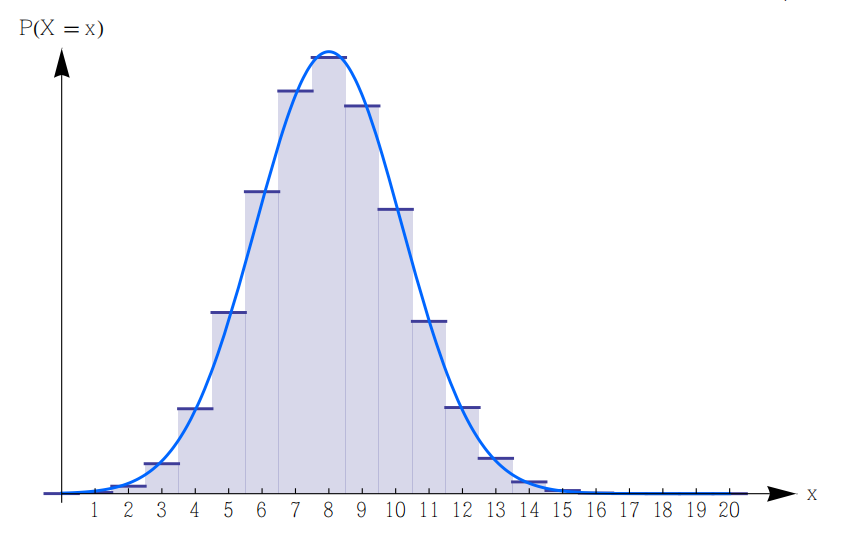
\includegraphics[scale=0.3]{appro.png}
\end{center}
\end{frame}


\begin{frame}{Normal Approximation of Binomial Distribution}
For $y=0, \ldots, n$
$$
P[X \leq y]=\sum_{x=0}^{y}\left(\begin{array}{l}
n \\
x
\end{array}\right) p^{x}(1-p)^{n-x} \approx \Phi\left(\frac{y+1 / 2-n p}{\sqrt{n p(1-p)}}\right)
$$
where we require that
$$
n p>5 \quad \text { if } p \leq \frac{1}{2} \quad \text { or } \quad n(1-p)>5 \quad \text { if } p>\frac{1}{2}
$$
This additional term $1 / 2$ is known as the \bb{half-unit correction} for the normal approximation to the \bb{cumulative} binomial distribution function.
\end{frame}


\begin{frame}{Central Limit Theorem}
\begin{block}{Theorem}
Central Limit Theorem. Let $\left(X_{i}\right)$ be a sequence of independent, but not necessarily identical random variables whose third moments exist and satisfy a certain technical condition. Let
$$
Y_{n}=X_{1}+\cdots+X_{n}
$$
Then for any $z \in \mathbb{R}$
$$
P\left[\frac{Y_{n}-\mathrm{E}\left[Y_{n}\right]}{\sqrt{\operatorname{Var}\left[Y_{n}\right]}} \leq z\right] \stackrel{n \rightarrow \infty}{\longrightarrow} \frac{1}{\sqrt{2 \pi}} \int_{-\infty}^{z} e^{-x^{2} / 2} d x
$$
\end{block}
\begin{block}{Interpretation}
Lyapunov’s Central Limit theorem is at the core of the belief by
experimentalists that “random error” may be described by the normal
distribution.
\end{block}
\end{frame}


\section{Multivariate Random Variables}
\subsection{Discrete, Continuous Multivariate R.V.}
\begin{frame}{Discrete Multivariate Random Variable}
\begin{block}{Definition}
Let $S$ be a sample space and $\Omega$ a countable subset of $\mathbb{R}^{n}$. A \bb{discrete multivariate random variable} is a map
$$
\mathbf{X}: S \rightarrow \Omega
$$
together with a function $f_{\mathbf{X}}: \Omega \rightarrow \mathbb{R}$ with the properties that
\begin{enumerate}
\item $f_{\mathbf{X}}(x) \geq 0$ for all $x=\left(x_{1}, \ldots, x_{n}\right) \in \Omega$ and
\item $\sum_{x \in \Omega} f_{\mathbf{X}}(x)=1$,
\end{enumerate}
where $f_{\mathbf{X}}$ is the \bb{joint density function} of the random variable $\mathbf{X}$.
\end{block}
\end{frame}

\begin{frame}{Discrete Multivariate Random Variable}
\begin{block}{Definition}
\begin{itemize}
\item \bb{Marginal density} $f_{X_{k}}$ for $X_{k}, k=1, \ldots, n$ :
$$
f_{X_{k}}\left(x_{k}\right)=\sum_{x_{1}, \ldots, x_{k-1}, x_{k+1}, \ldots, x_{n}} f_{X}\left(x_{1}, \ldots, x_{n}\right) .
$$
\item \bb{Independent} multivariate random variables:
$$
f_{\mathbf{X}}\left(x_{1}, \ldots, x_{n}\right)=f_{X_{1}}\left(x_{1}\right) \cdots f_{X_{n}}\left(x_{n}\right) .
$$
\item \bb{Conditional density} of $X_{1}$ conditioned on $X_{2}$ :
$$
f_{X_{1} \mid X_{2}}\left(x_{1}\right):=\frac{f_{X_{1} X_{2}}\left(x_{1}, x_{2}\right)}{f_{X_{2}}\left(x_{2}\right)} \quad \text { whenever } f_{X_{2}}\left(x_{2}\right)>0 .
$$
\end{itemize}
\end{block}
\end{frame}

\begin{frame}{Continuous Multivariate Random Variable}
\begin{block}{Definition}
Let $S$ be a sample space. A \bb{continuous multivariate random variable} is a map
$$
\mathbf{X}: S \rightarrow \mathbb{R}^{n}
$$
together with a function $f_{\mathbf{X}}: \mathbb{R}^{n} \rightarrow \mathbb{R}$ with the properties that
\begin{enumerate}
\item $f_{\mathbf{X}}(x) \geq 0$ for all $x=\left(x_{1}, \ldots, x_{n}\right) \in \mathbb{R}^{n}$ and
\item $\int_{\mathbb{R}^{n}} f_{\mathbf{X}}(x)=1$,
\end{enumerate}
where $f_{\mathbf{X}}$ is the \bb{joint density function} of the random variable $\mathbf{X}$.
\end{block}
\end{frame}

\begin{frame}{Continuous Multivariate Random Variable}
\begin{block}{Definition}
\begin{itemize}
\item \bb{Marginal density} $f_{X_{k}}$ for $X_{k}, k=1, \ldots, n$ :
$$
f_{X_{k}}\left(x_{k}\right)=\int_{\mathbb{R}^{n-1}} f_{X}\left(x_{1}, \ldots, x_{n}\right) \mathrm{d} x_{1} \ldots \mathrm{d} x_{k-1} \mathrm{~d} x_{k+1} \ldots \mathrm{d} x_{n} .
$$
\item \bb{Independent} multivariate random variables:
$$
f_{X}\left(x_{1}, \ldots, x_{n}\right)=f_{X_{1}}\left(x_{1}\right) \cdots f_{X_{n}}\left(x_{n}\right) .
$$
\item \bb{Conditional density} of $X_{1}$ conditioned on $X_{2}$ :
$$
f_{X_{1} \mid X_{2}}\left(x_{1}\right):=\frac{f_{X_{1} X_{2}}\left(x_{1}, x_{2}\right)}{f_{X_{2}}\left(x_{2}\right)} \quad \text { whenever } f_{X_{2}}\left(x_{2}\right)>0 \text {. }
$$
\end{itemize}
\end{block}
\end{frame}

\begin{frame}{Continuous Multivariate Random Variable}
\begin{block}{Example}
Suppose $Y$ is the rate (calls per hour) at which calls arrive at a switchboard. Let $X$ be the number of calls during a two-hour period. Suppose the joint probability density function is given by
$$f_{X Y}(x, y)= \begin{cases}\frac{(2 y)^{x}}{x !} e^{-3 y} & \text { for } y>0 \text { and } x=0,1, \ldots, \\ 0 & \text { otherwise }\end{cases}$$
\begin{itemize}
\item Verify that $f$ is a proper joint probability density function.
\item Find $P[X=0]$.
\end{itemize}
\end{block}
\end{frame}

\begin{frame}{Continuous Multivariate Random Variable}
\begin{block}{Solution}
\begin{itemize}
\item To verify that $f$ is a proper joint probability density function, we have
$$
\begin{aligned}
\int_{0}^{\infty}\left(\sum_{x=0}^{\infty} f_{X Y}(x, y)\right) d y &=\int_{0}^{\infty}\left(\sum_{x=0}^{\infty} \frac{(2 y)^{x}}{x !}\right) e^{-3 y} d y \\
&=\int_{0}^{\infty} e^{-y} d y \\
&=-\left.e^{-y}\right|_{0} ^{\infty}=1
\end{aligned}
$$
\item Plugging in $x=0$ and integrating with respect to $y$,
$$
P[X=0]=\int_{0}^{\infty} f_{X Y}(0, y) \mathrm{d} y=\int_{0}^{\infty} e^{-3 y} \mathrm{~d} y=\frac{1}{3} .
$$
\end{itemize}
\end{block}
\end{frame}

\begin{frame}{Continuous Multivariate Random Variable}
\begin{block}{Visualization}
Joint probability density function $f_{X Y}(x, y)$ (left)

conditional density function $f_{X \mid Y}\left(x \mid y_{0}\right)$ (right).
\begin{center}
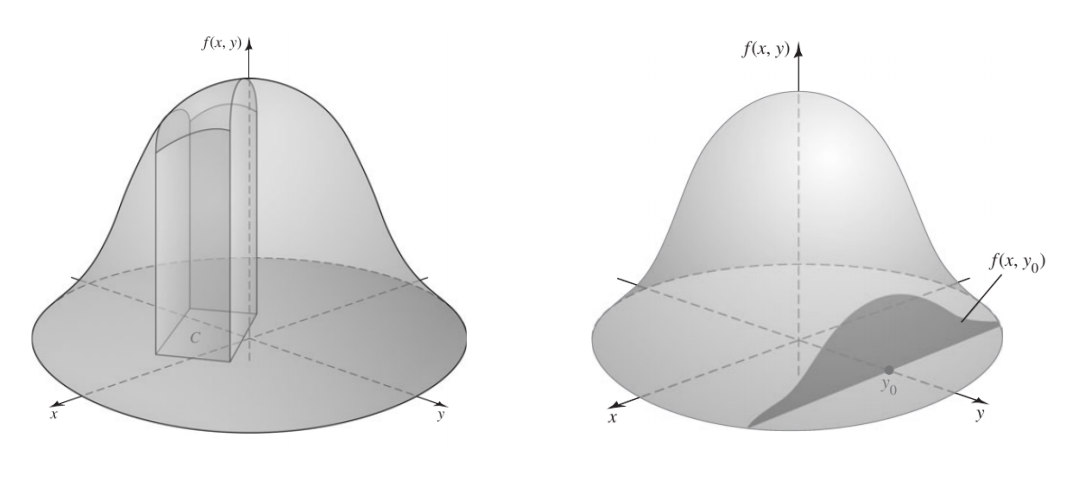
\includegraphics[scale=0.4]{vis.png}
\end{center}
\end{block}
\end{frame}

\begin{frame}{Continuous Multivariate Random Variable}
\begin{block}{Definition}
For continuous random variables $X_{1}, \ldots, X_{n}$, the \bb{joint cumulative distribution function} (CDF) is then given by
$$
P\left[X_{1} \leq a_{1}, \ldots, X_{n} \leq a_{n}\right]=\int_{-\infty}^{a_{1}} \cdots \int_{-\infty}^{a_{n}} f_{X}(x) \mathrm{d} x_{1} \ldots \mathrm{d} x_{n}
$$
\end{block}
\begin{block}{Example}
Suppose $X$ and $Y$ are random variables that take values in the intervals $0 \leq X \leq 2$ and $0 \leq Y \leq 2$. Suppose the joint cumulative distribution function for $x \in[0,2], y \in[0,2]$ is given by
$$
F(x, y)=\frac{1}{16} x y(x+y)
$$
What are the joint density function and cumulative distribution of $X ?$
\end{block}
\end{frame}


\begin{frame}{Continuous Multivariate Random Variable}
\begin{block}{Solution}
For $x \in[0,2], y \in[0,2]$
$$
f(x, y)=\frac{\partial^{2} F(x, y)}{\partial x \partial y}=\frac{1}{8}(x+y),
$$
and thus
$$
f_{X Y}(x, y)= \begin{cases}\frac{1}{8}(x+y) & 0 \leq x \leq 2,0 \leq y \leq 2 \\ 0 & \text { otherwise }\end{cases}
$$

Since for $y>2, F(x, y)=F(x, 2)$, then by letting $y \rightarrow \infty$, we obtain
$$
F_{X}(x)= \begin{cases}0 & x<0 \\ \frac{1}{8} x(x+2) & 0 \leq x \leq 2 \\ 1 & x>2\end{cases}
$$
\end{block}
\end{frame}


\subsection{Covariance and Correlation}
\begin{frame}{Expectation}
\begin{itemize}
\item Discrete.
$$
\mathrm{E}\left[X_{k}\right]=\sum_{x_{k}} x_{k} f_{X_{k}}\left(x_{k}\right)=\sum_{x \in \Omega} x_{k} f_{X}(x)
$$
and for continuous function $\varphi: \mathbb{R}^{n} \rightarrow \mathbb{R}$,
$$
\mathrm{E}[\varphi \circ \mathbf{X}]=\sum_{x \in \Omega} \varphi(x) f_{\mathbf{X}}(x)
$$
\item Continuous.
$$
\mathrm{E}\left[X_{k}\right]=\int_{\mathbb{R}} x_{k} f_{X_{k}}\left(x_{k}\right) \mathrm{d} x_{k}=\int_{\mathbb{R}^{n}} x_{k} f_{X}(x) \mathrm{d} x
$$
and for continuous function $\varphi: \mathbb{R}^{n} \rightarrow \mathbb{R}$,
$$
\mathrm{E}[\varphi \circ \mathbf{X}]=\int_{\mathbb{R}^{n}} \varphi(x) f_{\mathbf{X}}(x) \mathrm{d} x .
$$
\end{itemize}
\end{frame}


\begin{frame}{Covariance}
\begin{block}{Definition}
Definition. For a multivariate random variable $\mathbf{X}$, the \bb{covariance matrix} $\operatorname{Var}[\mathbf{X}]$ is given by
$$
\left(\begin{array}{cccc}
\operatorname{Var}\left[X_{1}\right] & \operatorname{Cov}\left[X_{1}, X_{2}\right] & \cdots & \operatorname{Cov}\left[X_{1}, X_{n}\right] \\
\operatorname{Cov}\left[X_{1}, X_{2}\right] & \operatorname{Var}\left[X_{2}\right] & \ddots & \vdots \\
\vdots & \ddots & \ddots & \operatorname{Cov}\left[X_{n-1}, X_{n}\right] \\
\operatorname{Cov}\left[X_{1}, X_{n}\right] & \cdots & \operatorname{Cov}\left[X_{n-1}, X_{n}\right] & \operatorname{Var}\left[X_{n}\right]
\end{array}\right)
$$
where the \bb{covariance} of $\left(X_{i}, X_{j}\right)$ is given by
$$
\operatorname{Cov}\left[X_{i}, X_{j}\right]=\mathrm{E}\left[\left(X_{i}-\mu_{X_{i}}\right)\left(X_{j}-\mu_{X_{j}}\right)\right]=\mathrm{E}\left[X_{i} X_{j}\right]-\mathrm{E}\left[X_{i}\right] \mathrm{E}\left[X_{j}\right]
$$
and
$$
\operatorname{Var}[\mathbf{C X}]=\mathbf{C} \operatorname{Var}[\mathbf{X}] \mathbf{C}^{T}, \quad \mathbf{C} \in \operatorname{Mat}(n \times n ; \mathbb{R})
$$
\end{block}
\end{frame}

\begin{frame}{Covariance}
\begin{block}{Properties}
Let $X, X_{1}, \ldots, X_{n}, Y$ and $Z$ be random variables.
\begin{itemize}
\item $X$ and $Y$ are independent $\Rightarrow \operatorname{Cov}[X, Y]=0$.

The Converse is not True!

\item $\operatorname{Var}[X+Y]=\operatorname{Var}[X]+\operatorname{Var}[Y]+2 \operatorname{Cov}[X, Y]$, and more generally,
$$
\begin{aligned}
\operatorname{Var}\left[X_{1}+\cdots+X_{n}\right]=\operatorname{Var}\left[X_{1}\right]+\cdots+& \operatorname{Var}\left[X_{n}\right]+2 \sum_{i<j} \operatorname{Cov}\left[X_{i}, X_{j}\right]
\end{aligned}
$$
if $\operatorname{Var}\left[X_{i}\right]<\infty$ for $i=1, \ldots, n$
\item $\operatorname{Cov}[X, Y+Z] = \operatorname{Cov}[X, Y] + \operatorname{Cov}[X, Z]$ 

$\operatorname{Cov}[X, Y-Z] = \operatorname{Cov}[X, Y] - \operatorname{Cov}[X, Z]$
\item $\operatorname{Cov}[X, X] = \operatorname{Var}[X]$
\end{itemize}
\end{block}
\end{frame}

\begin{frame}{Correlation}
\begin{block}{Definition}
The \bb{Pearson coefficient of correlation} of random variables $X$ and $Y$ is given by
$$
\rho_{X Y}:=\frac{\operatorname{Cov}[X, Y]}{\sqrt{\operatorname{Var}[X] \operatorname{Var}[Y]}}
$$
\end{block}
Instead of independence, the correlation coefficient actually measures the the extent to which $X$ and $Y$ are \bb{linearly} dependent, which is not the only way of being dependent.
\begin{block}{Properties}
\begin{itemize}
\item $-1 \leq \rho_{X Y} \leq 1$,
\item $\left|\rho_{X Y}\right|=1$ iff there exist $\beta_{0}, \beta_{1} \in \mathbb{R}$ such that
$$
Y=\beta_{0}+\beta_{1} X
$$
\end{itemize}
\end{block}
\end{frame}

\begin{frame}{Correlation}
\begin{block}{Note}
\begin{itemize}
\item Uncorrelated does not mean independent,
\item Correlation coefficient only measures linear relationships.
\end{itemize}
\end{block}
\begin{block}{Example}
Two random variables $X$ and $Y . X$ follows a uniform distribution $U(-1,1)$ and $Y=X^{2}$. Find $\operatorname{Cov}(X, Y)$.
$$
\begin{aligned}
\operatorname{Cov}(X, Y) &=\operatorname{Cov}\left(X, X^{2}\right) \\
&=\mathrm{E}\left((X-\mathrm{E}(X))\left(X^{2}-\mathrm{E}\left(X^{2}\right)\right)\right) \\
&=\mathrm{E}\left(X^{3}-X^{2} \mathrm{E}(X)-X \mathrm{E}\left(X^{2}\right)+\mathrm{E}(X) \mathrm{E}\left(X^{2}\right)\right) \\
&=\mathrm{E}\left(X^{3}\right)-\mathrm{E}\left(X^{2}\right) \mathrm{E}(X)-\mathrm{E}(X) \mathrm{E}\left(X^{2}\right)+\mathrm{E}(X) \mathrm{E}\left(X^{2}\right) \\
&=\int_{-1}^{1} \frac{1}{2} x^{3} \mathrm{~d} x-\int_{-1}^{1} \frac{1}{2} x^{2} \mathrm{~d} x \cdot \int_{-1}^{1} \frac{1}{2} x \mathrm{~d} x =0
\end{aligned}
$$
\end{block}
\end{frame}

\begin{frame}{Correlation}
\begin{block}{Example}
There is one more example. Suppose $X$ has a standard normal distribution. Let $W$ follows a distribution where $W=1$ or $W=-1$, each with probability $1 / 2$, and assume $W$ is independent of $X .$ Let $Y=W X$. Then
\begin{itemize}
\item $X$ and $Y$ are uncorrelated;
\item both have the same normal distribution; and
\item $X$ and $Y$ are not independent.
\end{itemize}

To see that $X$ and $Y$ are uncorrelated, by the independence of $W$ from $X$, one has
$$
\operatorname{cov}(X, Y)=\mathrm{E}(X Y)-0=\mathrm{E}\left(X^{2} W\right)=\mathrm{E}\left(X^{2}\right) \mathrm{E}(W)=\mathrm{E}\left(X^{2}\right) \cdot 0=0
$$
To see that $X$ and $Y$ are not independent, observe that $|Y|=|X|$
\end{block}
\end{frame}

\begin{frame}{The Fisher Transformation}
\begin{block}{Definition}
Let $\widetilde{X}$ and $\widetilde{Y}$ be standardized random variables of $X$ and $Y$, then the \bb{Fisher transformation} of $\rho_{X Y}$ is given by
$$\ln \left(\sqrt{\frac{\operatorname{Var}[\widetilde{X}+\widetilde{Y}]}{\operatorname{Var}[\widetilde{X}-\widetilde{Y}]}}\right)=\frac{1}{2} \ln \left(\frac{1+\rho_{X Y}}{1-\rho_{X Y}}\right)=\operatorname{Arctanh}\left(\rho_{X Y}\right) \in \mathbb{R}$$
We say that $X$ and $Y$ are
\begin{itemize}
\item \bb{positively correlated} if $\rho_{X Y}>0$, and
\item \bb{negatively correlated} if $\rho_{X Y}<0$.
\end{itemize}
\end{block}
\end{frame}

\begin{frame}{The Bivariate Normal Distribution}
The density function of \bb{Bivariate Normal Distribution}:
$$
f_{X Y}(x, y)=\frac{1}{2 \pi \sigma_{X} \sigma_{Y} \sqrt{1-\varrho^{2}}} e^{-\frac{1}{2\left(1-\varrho^{2}\right)}\left[\left(\frac{x-\mu_{X}}{\sigma_{X}}\right)^{2}-2 \varrho\left(\frac{x-\mu_{X}}{\sigma_{X}}\right)\left(\frac{y-\mu_{Y}}{\sigma_{Y}}\right)+\left(\frac{y-\mu_{Y}}{\sigma_{Y}}\right)^{2}\right]}
$$
\begin{itemize}
\item $-1<\varrho<1$
\item $\mu_{X}=\mathrm{E}[X], \sigma_{X}^{2}=\operatorname{Var} X$ (and similarly for $Y$ ).
\item $\varrho=\rho_{X Y}$ is indeed the correlation coefficient of $X$ and $Y$.
\item $X$ and $Y$ are independent $\Longleftrightarrow \varrho=0$
\end{itemize}
\end{frame}

\subsection{Hypergeometric Distribution}
\begin{frame}{Hypergeometric Distribution}
\begin{block}{Definition}
A random variable $\left(X, f_{X}\right)$ with parameters $N, n, r \in \mathbb{N} \backslash\{0\}$ where $r, n \leq N$ and $n<\min \{r, N-r\}$ has a \bb{hypergeometric distribution} if the density function is given by
$$
f_{X}(x)=\frac{\left(\begin{array}{l}
r \\
x
\end{array}\right)\left(\begin{array}{l}
N-r \\
n-x
\end{array}\right)}{\left(\begin{array}{l}
N \\
n
\end{array}\right)}
$$

\end{block}
\begin{block}{Interpretation}
\begin{itemize}
\item $f_{X}(x)$ is the probability of getting $x$ red balls in drawing $n$ balls from a box containing $N$ balls, where $r$ of them are red.
\item This can be formulated as obtaining $x$ successes in $n$ identical but not independent Bernoulli trials, each with probability of success $\frac{r}{N}$.
\end{itemize}
\end{block}
\end{frame}

\begin{frame}{Hypergeometric Distribution}
\begin{block}{Property}
\begin{itemize}
\item Expectation
$$
\mathrm{E}[X]=\mathrm{E}\left[X_{1}+\cdots+X_{n}\right]=n \frac{r}{N}
$$
\item Variance
$$
\begin{aligned}
\operatorname{Var}[X] &=\operatorname{Var}\left[X_{1}+\cdots+X_{n}\right] \\
&=\operatorname{Var}\left[X_{1}\right]+\cdots+\operatorname{Var}\left[X_{n}\right]+2 \sum_{i<j} \operatorname{Cov}\left[X_{i}, X_{j}\right] \\
&=n \frac{r}{N} \frac{N-r}{N} \frac{N-n}{N-1}
\end{aligned}
$$
\end{itemize}
The \bb{binomial distribution} may be used to approximate the hypergeometric distribution if $n / N$ is small (less than $0.05$).
\end{block}
\end{frame}

\begin{frame}{Hypergeometric Mean}
Transform to Bernoulli trials $\left(X_{1}, \ldots, X_{n}\right)$.

The Bernoulli trials are identical with $p_{k}=\frac{r}{N}$, i.e.,
$$
\begin{aligned}
P\left[X_{1}=1\right] &=\frac{r}{N} \\
P\left[X_{2}=1\right] &=P\left[X_{2}=1 \mid X_{1}=1\right] P\left[X_{1}=1\right]+\\
& \quad+P\left[X_{2}=1 \mid X_{1}=0\right] P\left[X_{1}=0\right] \\
&=\frac{r-1}{N-1} \cdot \frac{r}{N}+\frac{r}{N-1} \frac{N-r}{N} \\
&=\frac{r}{N}
\end{aligned}
$$
and so on.

\end{frame}

\begin{frame}{Hypergeometric Variance}
$$\begin{aligned}
\operatorname{Var}[X]=\operatorname{Var}\left[X_{1}\right]+\cdots+\operatorname{Var}\left[X_{n}\right]+2 \sum_{i<j} \operatorname{Cov}\left[X_{i}, X_{j}\right]
\end{aligned}$$
We need to calculate
$
\operatorname{Cov}\left[X_{i}, X_{j}\right]=\mathrm{E}\left[X_{i} X_{j}\right]-\mathrm{E}\left[X_{i}\right] \mathrm{E}\left[X_{j}\right] .
$
For this, we note that $X_{i} X_{j}$ is also a Bernoulli variable, since
$$
X_{i} X_{j}= \begin{cases}1 & \text { if } X_{i}=1 \text { and } X_{j}=1 \\ 0 & \text { otherwise }\end{cases}
$$
$$
\mathrm{E}\left[X_{i} X_{j}\right]=p_{i j}:=P\left[X_{i}=1 \text { and } X_{j}=1\right]=\frac{r}{N} \cdot \frac{r-1}{N-1}$$
$$
\operatorname{Var}\left[X_{i}\right]=\frac{r}{N}\left(1-\frac{r}{N}\right), \quad \operatorname{Cov}\left[X_{i}, X_{j}\right]=-\frac{1}{N} \cdot \frac{r(N-r)}{N(N-1)}
$$

Since there are $(\begin{array}{l}n \\ 2\end{array})$ pairs $(i, j)$ with $i<j$, finally gives
$$
\operatorname{Var}[X]=n \frac{r}{N} \frac{N-r}{N} \frac{N-n}{N-1}
$$
\end{frame}


\begin{frame}{Hypergeometric Distribution}
\begin{block}{Theorem}
Suppose $Y$ has a binomial distribution with parameters $n \in$ $\mathbb{N} \backslash\{0\}$ and $p, 0<p<1$. Let $\left\{X_{k}\right\}$ be a sequence of hypergeometric random variables with parameters $N_{k}, n, r_{k}$ such that
$$
\lim _{k \rightarrow \infty} N_{k}=\infty, \quad \lim _{k \rightarrow \infty} r_{k}=\infty, \quad \lim _{k \rightarrow \infty} \frac{r_{k}}{N_{k}}=p .
$$
Then for each fixed $n$ and each $x=0, \ldots, n$,
$$
\lim _{k \rightarrow \infty} \frac{P[Y=x]}{P\left[X_{k}=x\right]}=1
$$
\end{block}
\end{frame}

\begin{frame}{Hypergeometric Sample}
\begin{block}{Exercise}
Consider a group of $T$ people, and let $a_{1}, \ldots, a_{T}$ with mean $\mu$ and variance $\sigma^2$ denote the heights of these $T$ people. Suppose that $n$ people are selected from this group at random without replacement, and let $X$ denote the sum of heights of these $n$ persons. 

Determine the mean and variance of $X$.
\end{block}
\begin{block}{Solution}
Let $X_{i}$ be the height of the $i$-th person selected. Then $X=$ $X_{1}+\cdots+X_{n}$. Since $X_{i}$ is equally likely to have any one of the $T$ values, $\mathrm{E}\left[X_{i}\right]=\frac{1}{T} \sum_{i=1}^{T} a_{i}=\mu, \quad \operatorname{Var}\left[X_{i}\right]=\frac{1}{T} \sum_{i=1}^{T}\left(a_{i}-\mu\right)^{2}=\sigma^{2} .$
Therefore, $$E[X]=n \mu
\quad
\operatorname{Var}[X]=\sum_{i=1}^{n} \operatorname{Var}\left[X_{i}\right]+2 \sum_{i<j} \operatorname{Cov}\left[X_{i}, X_{j}\right]
$$
\end{block}
\end{frame}

\begin{frame}{Hypergeometric Sample}
\begin{block}{Solution}
How to solve Covariance?

Because $\operatorname{Cov}\left[X_{i}, X_{j}\right]$ does not depend on $i, j$ as long as $i \neq j$, we have
$$
\operatorname{Var}[X]=n \sigma^{2}+n(n-1) \operatorname{Cov}\left[X_{1}, X_{2}\right]
$$
Knowing that $\operatorname{Var}[X]=0$ for $n=T$, we have
$$
\begin{aligned}
\operatorname{Cov}\left[X_{1}, X_{2}\right]=-\frac{1}{T-1} \sigma^{2} \Rightarrow \operatorname{Var}[X] &=n \sigma^{2}-\frac{n(n-1)}{T-1} \sigma^{2} \\
&=n \sigma^{2}\left(\frac{T-n}{T-1}\right)
\end{aligned}
$$
\end{block}
\end{frame}

\subsection{Transformation of R.V. and Application}
\begin{frame}{Transformation of Random Variables}
\begin{block}{Theorem}
Let $\left(\boldsymbol{X}, f_{\boldsymbol{X}}\right)$ be a continuous multivariate random variable and let $\varphi: \mathbb{R}^{n} \rightarrow \mathbb{R}^{n}$ be a differentiable, bijective map with inverse $\varphi^{-1}$. Then $\boldsymbol{Y}=\varphi \circ \boldsymbol{X}$ is a continuous multivariate random variable with density
$$
f_{Y}(y)=f_{X} \circ \varphi^{-1}(y) \cdot\left|\operatorname{det} D \varphi^{-1}(y)\right|,
$$
where $D \varphi^{-1}$ is the Jacobian of $\varphi^{-1}$.
\end{block}
\begin{itemize}
\item $f_{Y}(y)=0$ for $y \notin \operatorname{ran} \varphi$.
\item When the map is not \bb{strictly monotonic}, we usually consider \bb{Cumulative Density Function}.
\item M.G.F. may help sometimes.
\end{itemize}
\end{frame}

\begin{frame}{Quotient of Normal: Cauchy}
\begin{block}{Lemma}
Let $\left((X, Y), f_{X Y}\right)$ be a continuous bivariate random variable. Let $U=X / Y$. Then the density $f_{U}$ of $U$ is given by
$$
f_{U}(u)=\int_{-\infty}^{\infty} f_{X Y}(u v, v) \cdot|v| d v .
$$
\end{block}
\begin{block}{Theorem}
Suppose that random variables $X$ and $Y$ are independent and that each follows the \bb{standard normal distribution}. Then $U=X / Y$ has the \bb{Cauchy distribution} with probability density function given by
$$
f_{U}(u)=\frac{1}{\pi\left(1+u^{2}\right)}, \quad u \in \mathbb{R} .
$$
\end{block}
\end{frame}

\begin{frame}{Quotient of Normal: Cauchy}
\begin{block}{Proof}
Let $V=Y$, excluding $Y=0$, the transformation from $(X, Y)$ to $(U, V)$ is one-to-one. Then $X=U V, Y=V$ and
$$
J=\operatorname{det}\left(\begin{array}{ll}
\frac{\partial x}{\partial u} & \frac{\partial x}{\partial v} \\
\frac{\partial y}{\partial u} & \frac{\partial y}{\partial v}
\end{array}\right)=v
$$
Then the joint density function is given by
$$
f_{U V}(u, v)=f_{X Y}(u v, v)|v|=\frac{|v|}{2 \pi} \exp \left(-\frac{1}{2}\left(u^{2}+1\right) v^{2}\right)
$$
Then the marginal of $U$ is calculated as
$$
f_{U}(u)=\int_{-\infty}^{\infty} f_{U v}(u, v) \mathrm{d} v=\frac{1}{\pi\left(u^{2}+1\right)}, \quad u \in \mathbb{R} .
$$
\end{block}
\end{frame}

\begin{frame}{Root Sum of Normal Square: Chi}
\begin{block}{Definition}
$\chi_{n}$ is a \bb{chi random variable} with $n$ \bb{degrees of freedom},
$$
\chi_{n}=\sqrt{\sum_{i=1}^{n} Z_{i}^{2}}
$$
where $Z_{1}, \ldots, Z_{n}$ are \bb{independent standard normal} random variables. 
$$f_{\chi_{n}}(y)=\frac{1}{2^{n / 2} \Gamma\left(\frac{n}{2}\right)} y^{n-1} e^{-y^2 / 2}\quad (y>0)$$
\end{block}

\begin{block}{Interpretation}
A chi random variable represents the sum of the root squares (distance) of independent standard normal variables.
\end{block}
\end{frame}



\begin{frame}{Sum of Normal Square: Chi-Squared}
\begin{block}{Definition}
$\chi_{n}^2$ is a \bb{chi-squared random variable} with $n$ \bb{degrees of freedom},
$$
\chi_{n}^{2}=\sum_{i=1}^{n} Z_{i}^{2}
$$
where $Z_{1}, \ldots, Z_{n}$ are \bb{independent standard normal} random variables. 
$$f_{\chi_{n}^{2}}(y)=\frac{1}{2^{n / 2} \Gamma\left(\frac{n}{2}\right)} y^{n / 2-1} e^{-y / 2}\quad (y>0)$$
\end{block}

\begin{block}{Interpretation}
A chi-squared random variable represents the sum of the squares of independent standard normal variables.
\end{block}
\end{frame}

\begin{frame}{Sum of Normal: Normal}
\begin{block}{Theorem}
If the random variables $X_{1}, \ldots, X_{k}$ are independent and if $X_{i}$ follows \bb{normal distribution} with mean $\mu_{i}$ and variance $\sigma_{i}^{2}$, where $i=1, \ldots, k$, then
$
X=X_{1}+\cdots+X_{k}
$
follows normal distribution with
$$
\mu=\mu_{1}+\cdots+\mu_{k}, \quad \sigma^{2}=\sigma_{1}^{2}+\cdots+\sigma_{k}^{2} .
$$
\end{block}
\begin{block}{Proof}
Using M.G.F., we have
$$
\begin{aligned}
m_{X}(t) &=\prod_{i=1}^{k} m_{X_{i}}(t)=\prod_{i=1}^{k} \exp \left(\mu_{i} t+\frac{1}{2} \sigma_{i}^{2} t^{2}\right) \\
&=\exp \left[\left(\sum_{i=1}^{k} \mu_{i}\right) t+\frac{1}{2}\left(\sum_{i=1}^{k} \sigma_{i}^{2}\right) t^{2}\right], \quad t \in \mathbb{R}
\end{aligned}
$$
\end{block}
\end{frame}

\begin{frame}{Sum of Chi-Squared: Chi-Squared}
\begin{block}{Lemma}
Let $\chi_{\gamma_{1}}^{2}, \ldots, \chi_{\gamma_{n}}^{2}$ be $n$ independent random variables following chi-squared distributions with $\gamma_{1}, \ldots, \gamma_{n}$ degrees of freedom, respectively. Then
$$
\chi_{\alpha}^{2}:=\sum_{k=1}^{n} \chi_{\gamma_{k}}^{2}
$$
is a \bb{chi-squared random variable} with $\alpha=\sum_{k=1}^{n} \gamma_{k}$ degrees of freedom.
\end{block}
\end{frame}

\section{Supplementary Materials}
\subsection{Discussion and Exercise}
\begin{frame}{1. Trigonometric Transformation}
\begin{block}{Exercise}
Let $(X, Y)$ be a continuous bivariate random variable with density $f_{X Y}: S \rightarrow \mathbb{R}^{2}$ given by
$$
f_{X Y}(x, y)= \begin{cases}c \cdot\left(x^{2}+y^{2}\right) & \text { for } x^{2}+y^{2} \leq 1 \\ 0 & \text { otherwise }\end{cases}
$$
where $c \in \mathbb{R}$ is a suitable constant.
\begin{enumerate}
\item Determine the constant $c$.
\item Find $\mathrm{E}[X]$ and $\mathrm{E}[Y]$.
\item Find $\operatorname{Var}[X]$ and $\operatorname{Var}[Y]$.
\item Find the correlation coefficient $\varrho_{X Y}$.
\end{enumerate}
\end{block}
\end{frame}

\begin{frame}{2. Not Bijective Map Transformation}
\begin{block}{Exercise}
(\bb{Univariate} R.V.) Let $X$ be a continuous \bb{uniformly distributed} random variable on $[-1,1]$. Does $X^2$ also follow uniform distribution?
\end{block}
\begin{block}{Exercise}
(\bb{Multivariate} R.V.) Let $(X, Y)$ be a continuous bivariate random variable with density $f_{X Y}: S \rightarrow \mathbb{R}^{2}$ given by
$$
f_{X Y}(x, y)= \begin{cases}\frac{2}{\pi} \cdot\left(x^{2}+y^{2}\right) & \text { for } x^{2}+y^{2} \leq 1 \\ 0 & \text { otherwise }\end{cases}
$$
Find the density of $U=X/Y$.
\end{block}
\end{frame}

\begin{frame}{3. Proof for Independence}
\begin{block}{Exercise}
Let $X, Y$ be independent random variables such that $X, Y \sim N\left(\mu, \sigma^{2}\right)$, show that $X+Y$ and $X-Y$ are independent.
\end{block}
Can we simply state that $$\operatorname{Cov}(X+Y,X-Y)=\operatorname{Cov}(X,X)+\operatorname{Cov}(X,Y)-\operatorname{Cov}(X,Y)-\operatorname{Cov}(Y,Y)$$
$$=\operatorname{Var}(X)-\operatorname{Var}(Y)=\sigma^2-\sigma^2=0$$
\end{frame}

\begin{frame}{4. Chi and Chi-Squared Distribution}
\begin{block}{Discussion}
How to derive Chi and \bb{Chi-Squared} distribution from \bb{Normal} Distribution?
\end{block}
\begin{block}{Exercise}
We can also derive \bb{Chi-Squared} following \bb{Uniform}-\bb{Exponential}-\bb{Gamma} thread.
\begin{enumerate}
\item Gamma distribution with parameters $\alpha=r,\beta=\lambda$ has M.G.F. $m_X(t)=\frac{1}{(1-t/\beta)^\alpha}$. What is the M.G.F. for Chi-squared distribution with $\gamma$ degrees of freedom?

\item If the random variables $X_{1}, X_{2}, \ldots, X_{n}$ are independent and follow the uniform distribution $U(0,1)$. Find the distribution of the random variable $Z=\sum_{i=1}^{n} Y_{i}$, where $Y=-2 \ln X$.
\end{enumerate}
\end{block}
\end{frame}

\newgeometry{left=0.01cm,bottom=0.5cm}
\begin{frame}
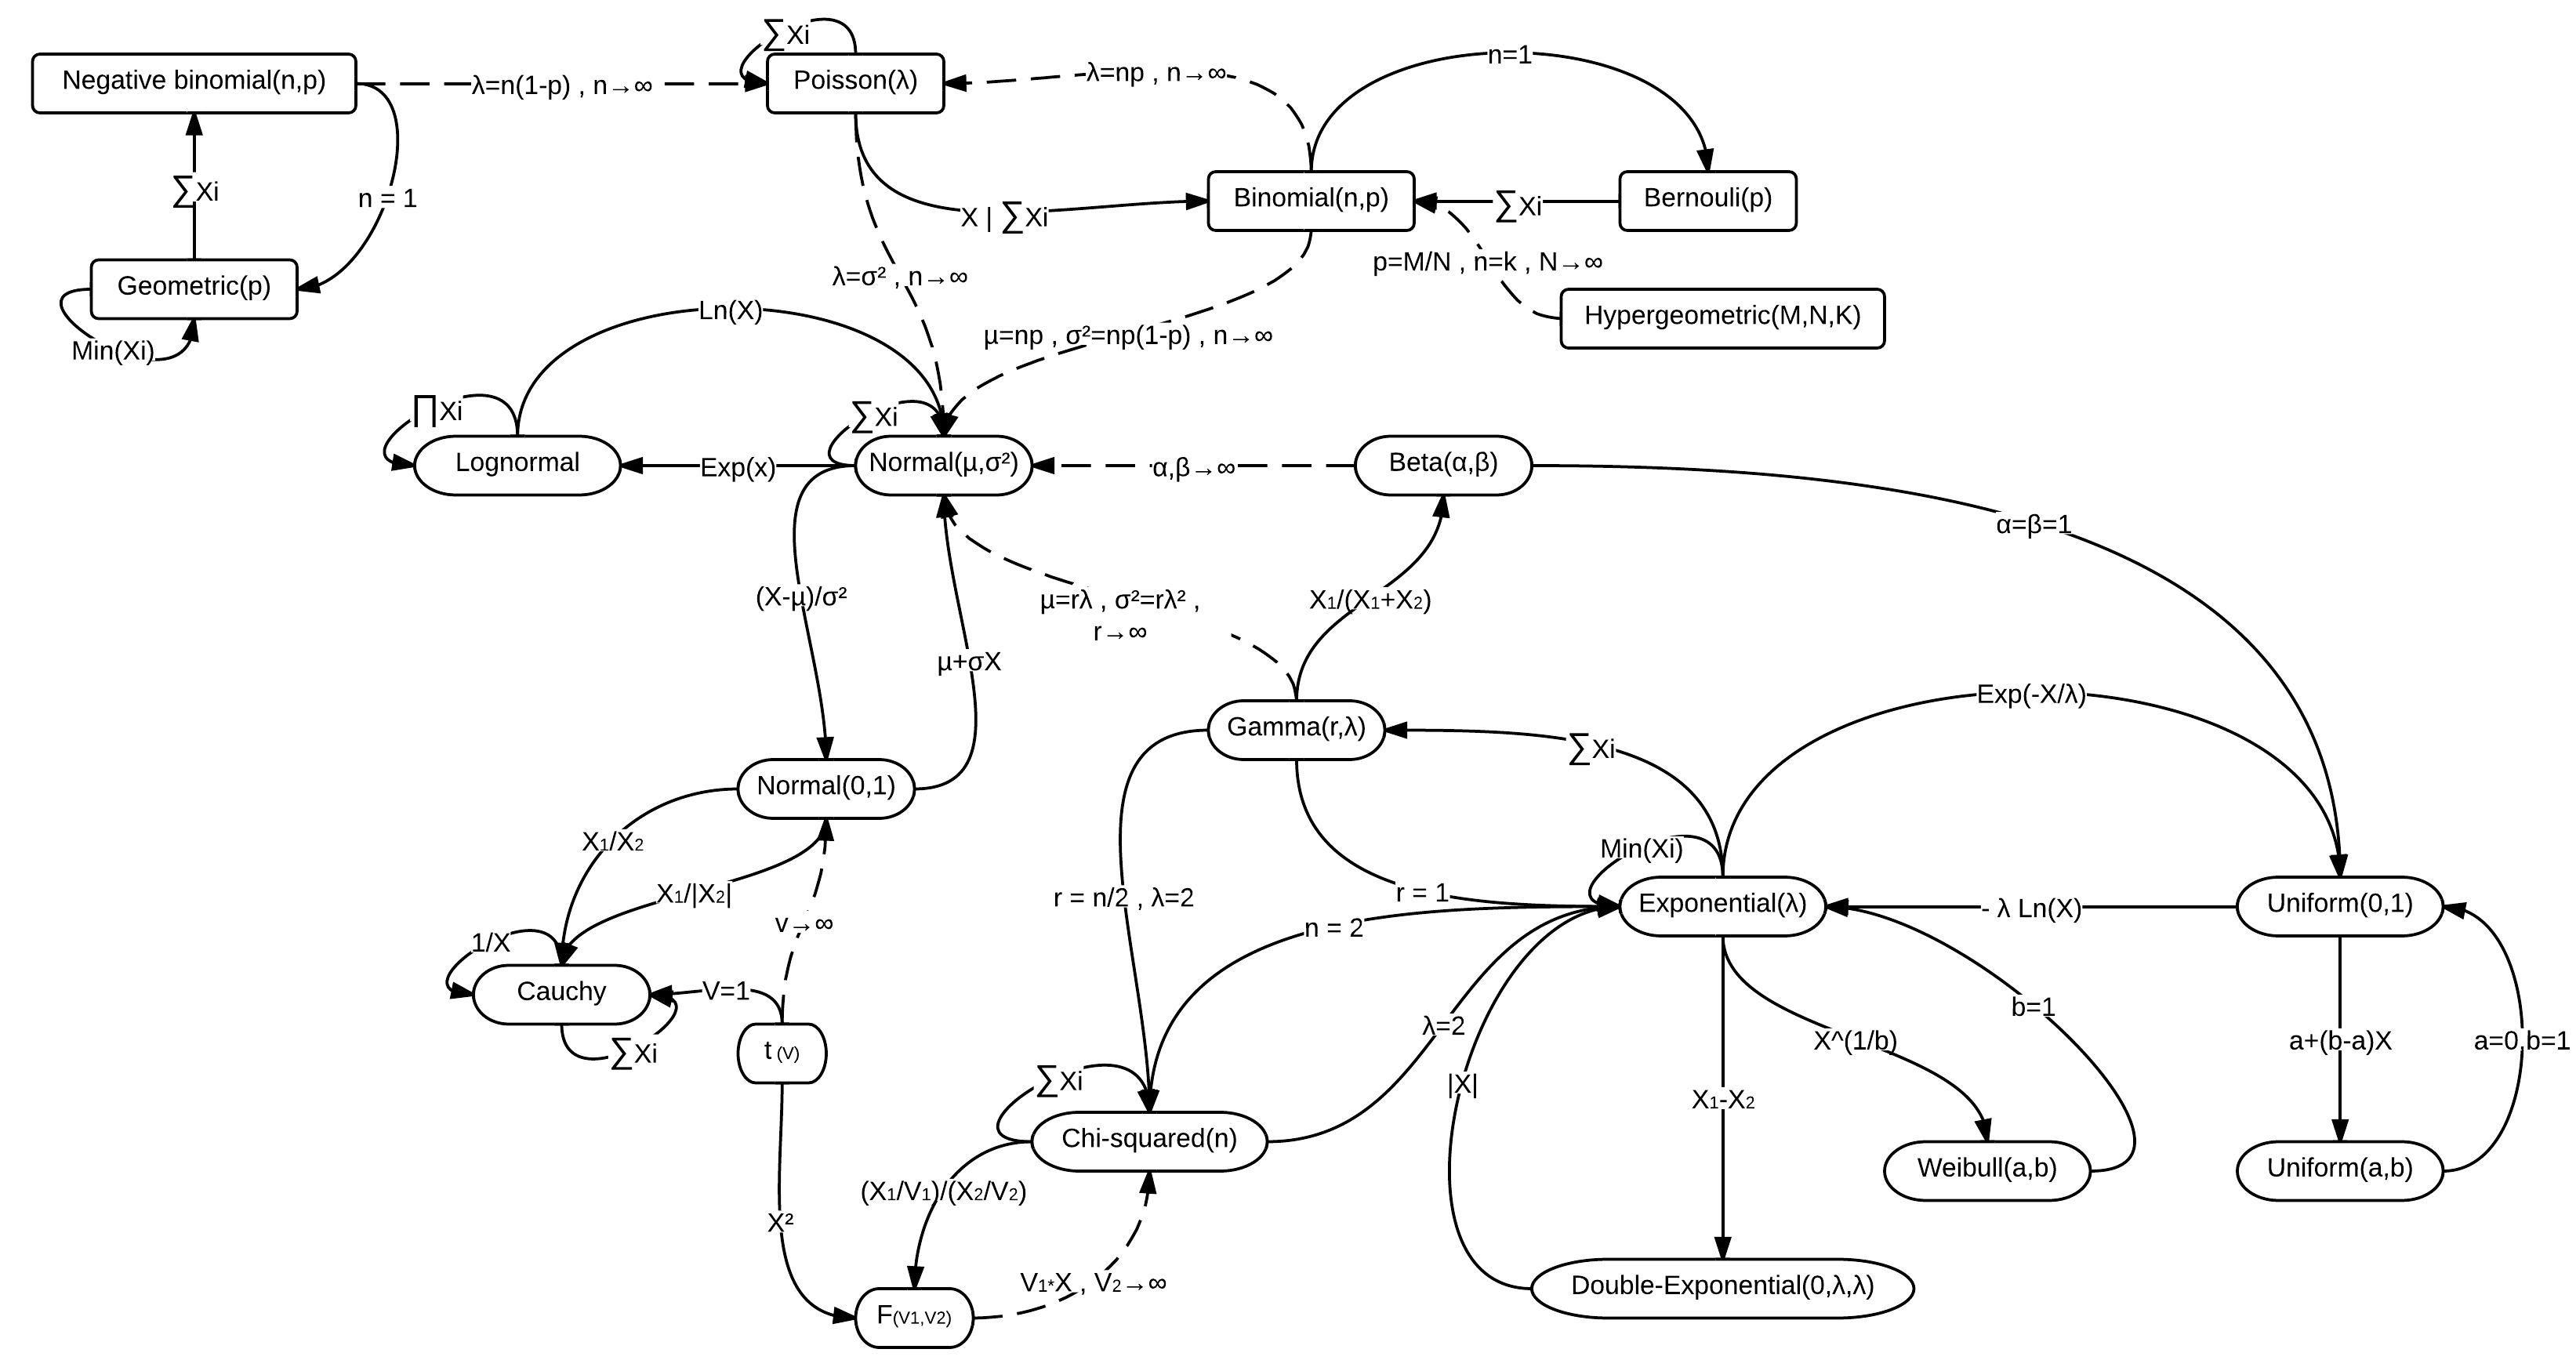
\includegraphics[scale=0.48]{diagram.jpg}
\end{frame}
\restoregeometry

\end{document}
%%Hyper变example,加一个CDF transform example,第三第四题